\documentclass[a4paper]{article}

\usepackage[french]{babel}
\usepackage[utf8]{inputenc}
\usepackage[T1]{fontenc}
\usepackage{fullpage}
\usepackage{hyperref}
\usepackage{graphicx}

\author{Titouan \bsc{Christophe}}
\title{Synthèse de bases de données}
\date{\today}

\begin{document}
\maketitle
\tableofcontents

\section{Modèle entité-relation}
Un schéma conceptuel des données, pas forcément implémenté de cette façon.

\subsection{Entité}
\begin{figure}[h!]
    \center
    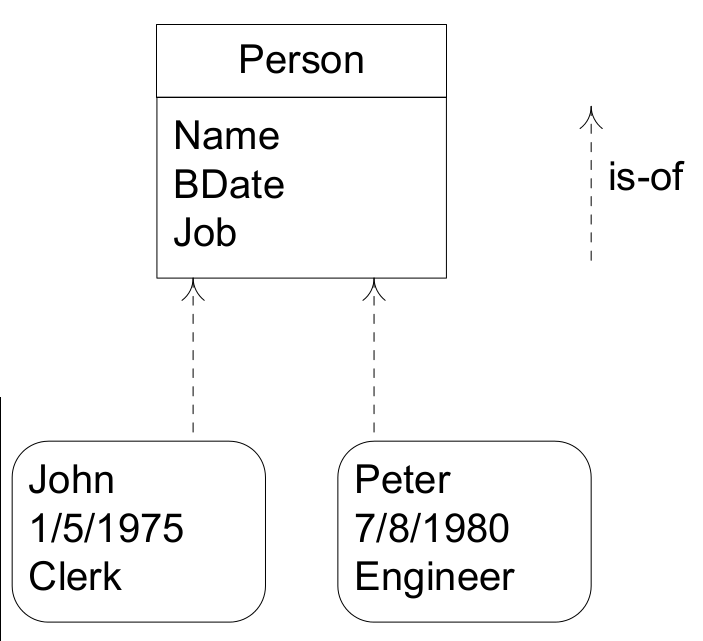
\includegraphics[width=.3\textwidth]{fig/entity.png}
    \caption{Une entité}
\end{figure}

Selon le contexte, désigne la classe (modèle) ou l'objet (l'instance).

\subsection{Relation}
\begin{figure}[h!]
    \center
    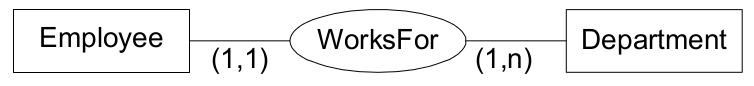
\includegraphics[width=.4\textwidth]{fig/relation.png}
    \caption{\label{fig:relation}Une relation One-to-many}
\end{figure}
\begin{figure}[h!]
    \center
    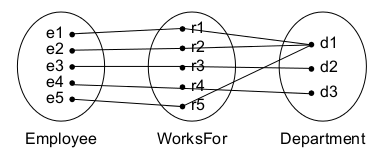
\includegraphics[width=.3\textwidth]{fig/relation-ensembliste.png}
    \caption{Vue ensembliste de la relation à la Figure \ref{fig:relation}}
\end{figure}
\begin{itemize}
  \item On doit spécifier la multiplicité minimale et maximale pour chaque pair de la relation
  \item La relation porte un nom (souvent lié au sens et à la sémantique de la relation)
  \item Une relation peut contenir des attributs
  \item L'arité ($x$-ary) d'une relation, ou son \textbf{degré}, indique le nombre d'entités participant à la relation
  \item \textbf{One-to-one}, \textbf{one-to-many} ou \textbf{many-to-many} pour les relations binaires
\end{itemize}

\subsubsection{Relation n-aire}
Une relation n-aire implique plus que 2 entités différentes.

\begin{figure}[h!]
    \center
    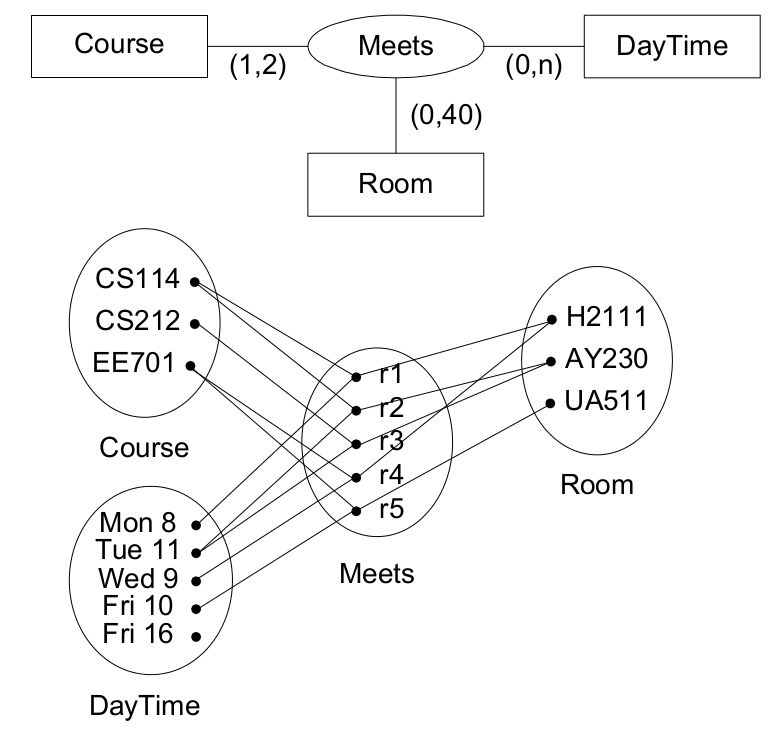
\includegraphics[width=.4\textwidth]{fig/relation-naire.png}
    \caption{Une relation ternaire et sa vue ensembliste}
\end{figure}

\paragraph{Transformation en relations binaires}
On peut transformer une relation $n$-aire en $n$ relations binaires par projection.
Cependant les relations obtenues après transformation contiennent moins d'information
que la relation initiale. Par exemple, dans la Figure \ref{fig:relation-naire-projection},
on voit que la relation ternaire indique qu'un fournisseur délivre un produit pour un projet,
tandis que les relations binaires indiquent uniquement qu'un fournisseur délivre un produit,
qu'un projet utilise un produit, et qu'un projet utilise un fournisseur.

\begin{figure}[h!]
    \center
    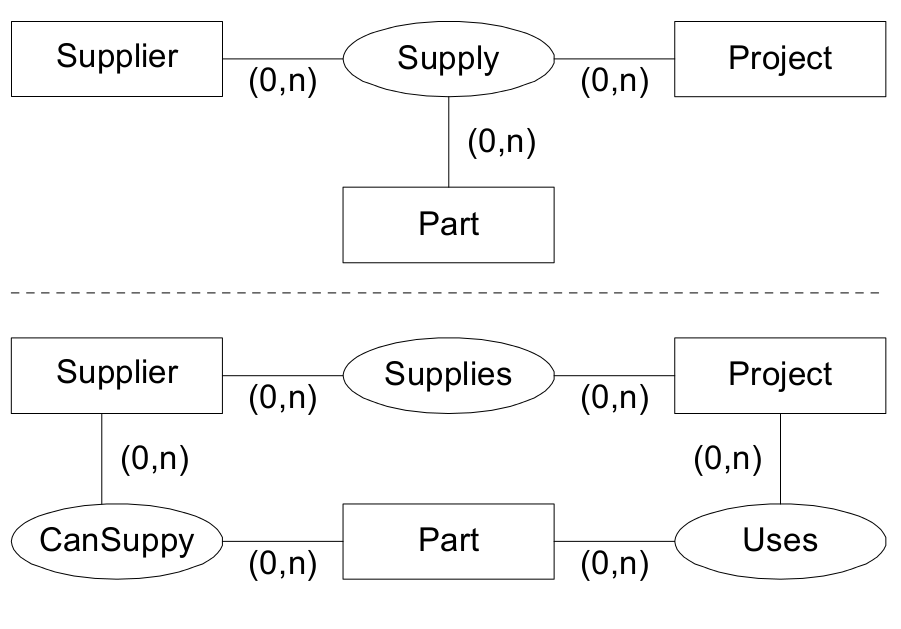
\includegraphics[width=.4\textwidth]{fig/relation-naire-projection.png}
    \caption{\label{fig:relation-naire-projection}Projection d'une relation ternaire}
\end{figure}

\end{document}